%% -*- coding:utf-8 -*-
\chapter{Natural transformation}

Natural transformation is the most important part of the category
theory. It provides a possibility to compare \mynameref{def:functor}s
via a standard tool. 

\section{Definitions}

The natural transformation is not an easy concept compare other ones
and requires some additional preparations before we can give the
formal definition.

\begin{figure}
  \centering
  \begin{tikzpicture}[ele/.style={fill=black,circle,minimum
        width=.8pt,inner sep=1pt},every fit/.style={ellipse,draw,inner
        sep=-2pt}]

    % the texts

    \node at (0,3) {$C$};        
    \node at (4,3) {$D$};        

    \node[ele,label=above:$a$] (a) at (0,2) {};    
    \node[ele,label=above:$a_F$] (af) at (4,2) {};
    \node[ele,label=below:$a_G$] (ag) at (4,0) {};

    \node[draw,fit= (a),minimum width=2cm, minimum
      height=3.5cm] {} ;
    \node[draw,fit= (af) (ag),minimum width=2cm, minimum
      height=3.5cm] {} ;

    \draw[->,thick,shorten <=2pt,shorten >=2pt] (a) to
    node[above]{$F$} (af);
    \draw[->,thick,shorten <=2pt,shorten >=2pt] (a) to
    node[above]{$G$} (ag);
    \draw[->,thick,shorten <=2pt,shorten >=2pt] (af) to
    node[right]{$\alpha_a$} (ag);
  \end{tikzpicture}
  \caption{Natural transformation: object mapping}
  \label{fig:nt_objects_mapping}
\end{figure}

Consider 2 categories $\cat{C}, \cat{D}$ and 2
\mynameref{def:functor}s $F: \cat{C} \tof \cat{D}$ and $G:
\cat{C} \tof \cat{D}$. If we have an \mynameref{def:object} $a \in \catob{C}$ then
it will be translated by different functors into different objects of
category $\cat{D}$: $a_F = F(a), a_G = G(a) \in \catob{D}$ (see
\cref{fig:nt_objects_mapping}). There are 2 options possible
\begin{enumerate}
\item There is not  any \mynameref{def:morphism} that connects $a_F$
  and $a_G$.
\item $\exists \alpha_a \in \hom\left(a_F, a_G\right) \subset
  \cathom{D}$. 
\end{enumerate}
We can of course to create an artificial morphism that connects the
objects but if we use \textit{natural} morphisms 
\footnote{the word natural means that already existent morphisms from
  category $\cat{D}$ are used}
then we can get a
special characteristic of the considered functors and categories. For
instance if we have such morphisms then we can say that the
considered functors are related each other. Opposite example if there
are no such morphisms then the functors can be considered as unrelated
each other. 
%% Another example if the
%% morphisms are \mynameref{def:isomorphism}s then the functors can be
%% considered as very close each other.

\begin{figure}
  \centering
  \begin{tikzpicture}[ele/.style={fill=black,circle,minimum
        width=.8pt,inner sep=1pt},every fit/.style={ellipse,draw,inner
        sep=-2pt}]

    % the texts

    \node at (0,3) {$C$};        
    \node at (4,3) {$D$};        

    \node[ele,label=above:$a$] (a) at (0,2) {};    
    \node[ele,label=below:$b$] (b) at (0,0) {};    
    \node[ele,label=above:$a_F$] (af) at (4,2) {};
    \node[ele,label=below:$a_G$] (ag) at (4,0) {};
    \node[ele,label=above:$b_F$] (bf) at (5.5,2) {};
    \node[ele,label=below:$b_G$] (bg) at (5.5,0) {};

    \node[draw,fit= (a) (b),minimum width=2cm, minimum
      height=3.5cm] {} ;
    \node[draw,fit= (af) (ag) (bf) (bg),minimum width=3cm, minimum
      height=4cm] {} ;

    \draw[->,thick,shorten <=2pt,shorten >=2pt] (a) to
    node[left]{$f$} (b);

    \draw[->,thick,shorten <=2pt,shorten >=2pt] (af) to
    node[below]{$f_F$} (bf);

    \draw[->,thick,shorten <=2pt,shorten >=2pt] (ag) to
    node[above]{$f_G$} (bg);

    \draw[->,thick,shorten <=2pt,shorten >=2pt] (a) to
    node[above]{$F$} (af);
    \draw[->,thick,shorten <=2pt,shorten >=2pt] (b) to
    [out=45,in=135,looseness=1] node[above]{$F$} (bf);
    \draw[->,thick,shorten <=2pt,shorten >=2pt] (a) to
    node[above]{$G$} (ag);
    \draw[->,thick,shorten <=2pt,shorten >=2pt] (b) to
    [out=-45,in=-135,looseness=1] node[above]{$G$} (bg);
    \draw[->,thick,shorten <=2pt,shorten >=2pt] (af) to
    node[left]{$\alpha_a$} (ag);
    \draw[->,thick,shorten <=2pt,shorten >=2pt] (bf) to
    node[right]{$\alpha_b$} (bg);
  \end{tikzpicture}
  \caption{Natural transformation: morphisms mapping}
  \label{fig:nt_morphisms_mapping}
\end{figure}


The functor is not just the object mapping but also the morphisms
mapping. If we have 2 objects $a$ and $b$ in the category $\cat{C}$
then we potentially can have a morphism $f \in \hom_{\cat{C}}(a, b)$. In this
case the morphism is mapped by the functors $F$ and $G$ into 2
morphisms $f_f$ and $f_G$ in the category $\cat{D}$. 
As result we have 4 morphisms: $\alpha_a, \alpha_b, f_F, f_G \in
\cathom{D}$. It is natural to impose additional conditions on the
morphisms especially that they form a
\mynameref{def:commutative_diagram} (see \cref{fig:nt_def}): 
\[
f_f \circ \alpha_b = \alpha_a \circ f_G.
\]

\begin{definition}[Natural transformation]
\label{def:nt}

\begin{figure}
  \centering
  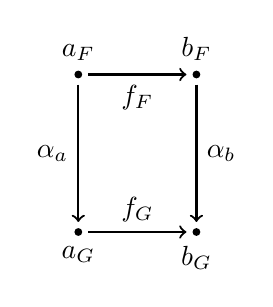
\begin{tikzpicture}[ele/.style={fill=black,circle,minimum
        width=.8pt,inner sep=1pt},every fit/.style={ellipse,draw,inner
        sep=-2pt}]

    % the texts
    \node[ele,label=above:$a_F$] (af) at (0,2) {};
    \node[ele,label=below:$a_G$] (ag) at (0,0) {};
    \node[ele,label=above:$b_F$] (bf) at (1.5,2) {};
    \node[ele,label=below:$b_G$] (bg) at (1.5,0) {};

    \draw[->,thick,shorten <=2pt,shorten >=2pt] (af) to
    node[below]{$f_F$} (bf);
    \draw[->,thick,shorten <=2pt,shorten >=2pt] (ag) to
    node[above]{$f_G$} (bg);
    \draw[->,thick,shorten <=2pt,shorten >=2pt] (af) to
    node[left]{$\alpha_a$} (ag);
    \draw[->,thick,shorten <=2pt,shorten >=2pt] (bf) to
    node[right]{$\alpha_b$} (bg);
  \end{tikzpicture}
  \caption{Natural transformation: commutative diagram}
  \label{fig:nt_def}
\end{figure}

Let $F$ and $G$ are 2 \mynameref{def:functor}s from category $\cat{C}$
to the category $\cat{D}$. The \textit{natural transformation} is a
set of \mynameref{def:morphism}s $\alpha \subset \cathom{D}$ which
satisfy the following conditions:
\begin{itemize}
\item For every \mynameref{def:object} $a \in \catob{C}$ $\exists
\alpha_a \in \hom\left(a_F, a_G\right)$
\footnote{
$a_F = F(a), a_G = G(a)$
}
- \mynameref{def:morphism}
in category $\cat{D}$. The morphism $\alpha_a$ is called the component of
the natural transformation.
\item For every morphism $f \in \cathom{C}$ that connects 2 objects
  $a$ and $b$, i.e. $f \in \hom_{\cat{C}}(a,b)$ the corresponding components of
  the natural transformation $\alpha_a, \alpha_b \in \alpha$ should
  satisfy the following conditions
  \begin{equation}
    f_G \circ \alpha_a = \alpha_b \circ f_F,
    \label{eq:nt_definition}
  \end{equation}
  where $f_F = F(f), f_G = G(f)$.
  In other words the morphisms form a
  \mynameref{def:commutative_diagram} shown on the \cref{fig:nt_def}. 
\end{itemize}

We use the following notation (arrow with a dot) for the natural transformation between
functors $F$ and $G$: $\alpha: F \tont G$. 
\end{definition}

\section{Operations with natural transformations}

\begin{example}[\textbf{Fun} category]
%% \label{ex:fun_category}
%% \index{Object!\textbf{Fun} example}
%% \index{Morphism!\textbf{Fun} example}
%% \index{Category!\textbf{Fun} example}

%% The functors can be considered as objects in a special category
%% \textbf{Fun}. The morphisms in the category are \mynameref{def:nt}s.

%% To define a category we need to define composition operation that
%% satisfied \mynameref{axm:composition}, identity
%% morphism and verify \mynameref{axm:associativity}. 

%% \begin{figure}
%%   \centering
%%   \begin{tikzpicture}[ele/.style={fill=black,circle,minimum
%%         width=.8pt,inner sep=1pt},every fit/.style={ellipse,draw,inner
%%         sep=-2pt}]

%%     % the texts

%%     \node at (0,3) {$C$};        
%%     \node at (4,5) {$D$};        

%%     \node[ele,label=above:$a$] (a) at (0,2) {};    
%%     \node[ele,label=above:$a_F$] (af) at (4,4) {};
%%     \node[ele,label=right:$a_G$] (ag) at (4,2) {};
%%     \node[ele,label=below:$a_H$] (ah) at (4,0) {};

%%     \node[draw,fit= (a),minimum width=2cm, minimum
%%       height=3.5cm] {} ;
%%     \node[draw,fit= (af) (ag) (ah),minimum width=5cm, minimum
%%       height=5cm] {} ;

%%     \draw[->,thick,shorten <=2pt,shorten >=2pt] (a) to
%%     node[above]{$F$} (af);
%%     \draw[->,thick,shorten <=2pt,shorten >=2pt] (a) to
%%     node[above]{$G$} (ag);
%%     \draw[->,thick,shorten <=2pt,shorten >=2pt] (a) to
%%     node[above]{$H$} (ah);
%%     \draw[->,thick,shorten <=2pt,shorten >=2pt] (af) to
%%     node[right]{$\alpha_a$} (ag);
%%     \draw[->,thick,shorten <=2pt,shorten >=2pt] (ag) to
%%     node[right]{$\beta_a$} (ah);
%%     \draw[->,thick,shorten <=2pt,shorten >=2pt] (af) to
%%      [out=-45,in=45,looseness=1] node[right]{$\beta_a \circ \alpha_a$} (ah);
%%   \end{tikzpicture}
%%   \caption{Natural transformation vertical composition: object mapping}
%%   \label{fig:nt_objects_mapping_composition}
%% \end{figure}


%% For the composition consider 2 \mynameref{def:nt}s $\alpha, \beta$ and
%% consider how they act on an object $a \in \catob{C}$ (see
%% \cref{fig:nt_objects_mapping_composition}). We always can construct
%% the composition $\beta_a \circ \alpha_a$ i.e. we can define the
%% composition of natural transformations $\alpha, \beta$ as 
%% \(
%% \beta \circ \alpha = \left\{
%% \beta_a \circ \alpha_a | a \in \catob{C}
%% \right\}
%% \). 

%% \begin{figure}
%%   \centering
%%   \begin{tikzpicture}[ele/.style={fill=black,circle,minimum
%%         width=.8pt,inner sep=1pt},every fit/.style={ellipse,draw,inner
%%         sep=-2pt}]

%%     % the texts

%%     \node[ele,label=above:$a_F$] (af) at (0,4) {};
%%     \node[ele,label=left:$a_G$] (ag) at (0,2) {};
%%     \node[ele,label=below:$a_H$] (ah) at (0,0) {};
%%     \node[ele,label=above:$b_F$] (bf) at (3,4) {};
%%     \node[ele,label=right:$b_G$] (bg) at (3,2) {};
%%     \node[ele,label=below:$b_H$] (bh) at (3,0) {};

%%     \draw[->,thick,shorten <=2pt,shorten >=2pt] (af) to
%%     node[above]{$f_F$} (bf);
%%     \draw[->,thick,shorten <=2pt,shorten >=2pt] (ag) to
%%     node[above]{$f_G$} (bg);
%%     \draw[->,thick,shorten <=2pt,shorten >=2pt] (ah) to
%%     node[above]{$f_H$} (bh);

%%     \draw[->,thick,shorten <=2pt,shorten >=2pt] (af) to
%%     node[right]{$\alpha_a$} (ag);
%%     \draw[->,thick,shorten <=2pt,shorten >=2pt] (ag) to
%%     node[right]{$\beta_a$} (ah);
%%     \draw[->,thick,shorten <=2pt,shorten >=2pt] (af) to
%%      [out=-135,in=135,looseness=1] node[left]{$\beta_a \circ
%%        \alpha_a$} (ah);
%%     \draw[->,thick,shorten <=2pt,shorten >=2pt] (bf) to
%%     node[right]{$\alpha_b$} (bg);
%%     \draw[->,thick,shorten <=2pt,shorten >=2pt] (bg) to
%%     node[right]{$\beta_b$} (bh);
%%     \draw[->,thick,shorten <=2pt,shorten >=2pt] (bf) to
%%      [out=-45,in=45,looseness=1] node[right]{$\beta_b \circ \alpha_b$}
%%      (bh); 
%%   \end{tikzpicture}
%%   \caption{Natural transformation vertical composition: morphism mapping -
%%     commutative diagram}
%%   \label{fig:nt_morphism_mapping_composition}
%% \end{figure}


%% The natural transformation is not just object mapping but also
%% morphism mapping. We will require that all morphisms shown on
%% \cref{fig:nt_morphism_mapping_composition} commute. 
%% The composition 
%% defined in such way is called \mynameref{def:vertical_composition}.  

%% The functor category between categories $\cat{C}$ and $\cat{D}$ is
%% denoted as $[\cat{C}, \cat{D}]$.

\end{example}

\begin{definition}[Vertical composition]
\label{def:vertical_composition}
\index{Natural transformation!Vertical composition}
Let $F,G,H$ are functors between categories $\cat{C}$ and $\cat{D}$.
Also we have $\alpha : F \tont G, \beta: G \tont
H$ - natural transformations. We can compose the $\alpha$ and $\beta$
as follows 
\[
\alpha \circ \beta: F \tont H.
\]
This composition
is called \textit{vertical composition}.
\end{definition}

\begin{definition}[Horizontal composition]
\label{def:horizontal_composition}
\index{Natural transformation!Horizontal composition}
If we have 2 pairs of functors. The first one $F,G: \cat{C} \to
\cat{D}$ and another one $J,K: \cat{D} \tof \cat{E}$. We also have a
natural transformation between each pair: $\alpha : F \tont
G$ for the first one and $\beta : J \tont
K$ for the second one. We can create a new transformation
\[
\alpha \star \beta: F \circ J \tont G \circ K
\] 
that is called \textit{horizontal composition}. Note that we use a
special symbol $\star$ for the composition.
\end{definition}

\begin{remark}[Bifunctor in category of functors]
 \label{rem:bifunctor_fun_cat}
If we have the same pair of functors as in
\cref{def:horizontal_composition} then we can consider the functors as
objects of 3 categories: $\cat{\mathcal{A}} = \left[\cat{C},
  \cat{D}\right], \cat{\mathcal{B}} = \left[\cat{D},
  \cat{E}\right]$ and $\cat{\mathcal{C}} = \left[\cat{C},
  \cat{E}\right]$ 

  Next we want to construct a \mynameref{def:bifunctor} 
  $\otimes: \cat{\mathcal{A}} \times \cat{\mathcal{B}} \tof \cat{\mathcal{C}}$
  where for each pair of objects $F \in \catob{\mathcal{A}}, J \in
  \catob{\mathcal{B}}$ we got another object from $\cat{\mathcal{C}}$.
  The used operation is an ordinary functor's composition.
  I.e.
  \[
  \otimes: F \times G \to F \circ G \in \catob{\mathcal{C}}.
  \]
  
  The bifunctor is not just a map for objects. There is also a map
  between morphisms. Thus if we have 2 \mynameref{def:morphism}s:
  $\alpha : F \to G$ and $\beta : J \to K$ then we can construct the
  following mapping 
  \[
  \otimes: \alpha \times \beta \to \alpha \star \beta \in \cathom{\mathcal{C}}.
  \]
  
  As result we have the introduced mapping $\otimes$ as a bifunctor.
\end{remark}

\begin{definition}[Left whiskering]
\label{def:lw}
If we have 3 categories $\cat{B}, \cat{C}, \cat{D}$, 
\mynameref{def:functor}s $F,G: \cat{C} \tof \cat{D}$, $H: \cat{B} \to
\cat{C}$ and \mynameref{def:nt} 
$\alpha: F \tont G$ then we can construct a new natural
transformations:
\[
\alpha H : F \circ H \tont G \circ H
\]
that is called \textit{left whiskering} of functor and natural
transformation \cite{nlab:whiskering}. 
\end{definition}

\begin{definition}[Right whiskering]
\label{def:rw}
If we have 3 categories $\cat{C}, \cat{D}, \cat{E}$, 
\mynameref{def:functor}s $F,G: \cat{C} \tof \cat{D}$, $H: \cat{D} \to
\cat{E}$ and \mynameref{def:nt} 
$\alpha: F \tont G$ then we can construct a new natural 
transformations: 
\[
H \alpha : H \circ F \tont H \circ G
\]
that is called \textit{right whiskering} of functor and natural
transformation \cite{nlab:whiskering}. 
\end{definition}

\begin{definition}[Identity natural transformation]
\label{def:idnt}
If $F: \cat{C} \tof \cat{D}$ is a \mynameref{def:functor} then we can
define \textit{identity natural transformation}
$\idnt{F}$ that maps any \mynameref{def:object} 
$a \in \catob{C}$ into \mynameref{def:id} $\idm{F(a)} \in \cathom{D}$.
\end{definition}

\begin{remark}[Whiskering]
\label{rem:whiskering}
With \mynameref{def:idnt} we can redefine \mynameref{def:lw} and
\mynameref{def:rw} via \mynameref{def:horizontal_composition} as follows.

For left whiskering:
\begin{equation}
\label{eq:lw}
\alpha H = \alpha \star \idnt{H}
\end{equation}

For right whiskering:
\begin{equation}
\label{eq:rw}
H \alpha = \idnt{H} \star \alpha
\end{equation}
\end{remark}


\section{Polymorphism and natural transformation}

Polymorphism plays a certain role in programming languages. Category
theory provides several facts about polymorphic functions which are
very important.

\begin{definition}[Parametrically polymorphic function]
\index{Parametric polymorphism}
\label{def:pp_function}
Polymorphism is parametric if all function instances behave uniformly
i.e. have the same realization. The functions which satisfy the
parametric polymorphism requirements are parametrically polymorphic.
\end{definition}

\begin{definition}[Ad-hoc polymorphism]
\label{def:ad_hoc_polymorphism}
Polymorphism is parametric if the function instances can behave
differently dependently on the type they are being instantiated with. 
\end{definition}

\begin{theorem}[Reynolds]
\label{thm:reynolds}
\mynameref{def:pp_function}s are \mynameref{def:nt}s 
\begin{proof}
TBD
\end{proof}
\end{theorem}

\subsection{\textbf{Hask} category}

In Haskell most of functions are \mynameref{def:pp_function}s 
\footnote{really in the run-time the functions are not
  \mynameref{def:pp_function}s}.  

\begin{example}[Parametrically polymorphic function][\textbf{Hask}]
\label{ex:nt_hask}
Consider the following function
\begin{minted}{haskell}
safeHead :: [a] -> Maybe a
safeHead [] = Nothing
safeHead (x:xs) = Just x
\end{minted}
The function is parametricaly polymorphic and by
\mynameref{thm:reynolds} is \mynameref{def:nt} (see \cref{fig:nt_pp_hask}).

\begin{figure}
  \centering
  \begin{tikzpicture}[ele/.style={fill=black,circle,minimum
        width=.8pt,inner sep=1pt},every fit/.style={ellipse,draw,inner
        sep=-2pt}]

    % the texts

    \node[ele,label=above:$a$] (a) at (0,2) {};    
    \node[ele,label=below:$b$] (b) at (0,0) {};    
    \node[ele,label=above:$\mbox{[a]}$] (af) at (5,2) {};
    \node[ele,label=below:$\mbox{Maybe a}$] (ag) at (5,0) {};
    \node[ele,label=above:$\mbox{[b]}$] (bf) at (7.5,2) {};
    \node[ele,label=below:$\mbox{Maybe b}$] (bg) at (7.5,0) {};

    \node[draw,fit= (a) (b),minimum width=2cm, minimum
      height=3.5cm] {} ;
    \node[draw,fit= (af) (ag) (bf) (bg),minimum width=6.5cm, minimum
      height=5.5cm] {} ;

    \draw[->,thick,shorten <=2pt,shorten >=2pt] (a) to
    node[left]{$f$} (b);

    \draw[->,thick,shorten <=2pt,shorten >=2pt] (af) to
    node[below]{$\mbox{fmap}_{[]}$} (bf);

    \draw[->,thick,shorten <=2pt,shorten >=2pt] (ag) to
    node[above]{$\mbox{fmap}_{Maybe}$} (bg);

    \draw[->,thick,shorten <=2pt,shorten >=2pt] (a) to
    node[above]{$$} (af);
    \draw[->,thick,shorten <=2pt,shorten >=2pt] (b) to
    [out=45,in=135,looseness=1] node[above]{$$} (bf);
    \draw[->,thick,shorten <=2pt,shorten >=2pt] (a) to
    node[above]{$$} (ag);
    \draw[->,thick,shorten <=2pt,shorten >=2pt] (b) to
    [out=-45,in=-135,looseness=1] node[above]{$$} (bg);
    \draw[->,thick,shorten <=2pt,shorten >=2pt] (af) to
    node[left]{$\mbox{safeHead}_a$} (ag);
    \draw[->,thick,shorten <=2pt,shorten >=2pt] (bf) to
    node[right]{$\mbox{safeHead}_b$} (bg);
  \end{tikzpicture}
  \caption{Haskell parametric polymorphism as a natural transformation}
  \label{fig:nt_pp_hask}
\end{figure}

Therefore from the definition of the natural transformation
\eqref{eq:nt_definition} we have 
\textbf{fmap f . safeHead = safeHead . fmap f}. I.e. it
does not matter if we initially apply \textbf{fmap f} and
then \textbf{safeHead} to the result or initially
\textbf{safeHead} and then \textbf{fmap f}.

The statement can be verified directly. For empty list we have
\begin{minted}{haskell}
fmap f . safeHead []
-- equivalent to
fmap f Nothing 
-- equivalent to
Nothing
\end{minted}
from other side
\begin{minted}{haskell}
safeHead . fmap f []
-- equivalent to
safeHead [] 
-- equivalent to
Nothing
\end{minted}

For a non empty list we have
\begin{minted}{haskell}
fmap f . safeHead (x:xs)
-- equivalent to
fmap f (Just x) 
-- equivalent to
Just (f x)
\end{minted}
from other side
\begin{minted}{haskell}
safeHead . fmap f (x:xs)
-- equivalent to
safeHead (f x: fmap f xs ) 
-- equivalent to
Just ( f x )
\end{minted}

Using the fact that \textbf{fmap f} is an expensive
operation if it is applied to the list we can conclude that the second
approach is more productive. Such transformation allows compiler to
optimize the code.
\footnote{It is not directly applied to Haskell because it has lazy
  evaluation that can perform optimization before that one}
\end{example}
